\documentclass[11pt,a4paper]{article}
\usepackage[margin=1in, headheight=14pt]{geometry}
\usepackage{amsfonts,amsmath,amssymb,suetterl}
\usepackage{lmodern}
\usepackage[T1]{fontenc}
\usepackage{fancyhdr}
\usepackage{float}
\usepackage[utf8]{inputenc}
\usepackage{fontawesome}
\usepackage{enumerate}
\usepackage{xcolor}
\usepackage{hyperref}
\usepackage{tikz}
\usepackage{nicefrac}
\usepackage{subcaption}
\usepackage{physics}
\usepackage{mathtools}
\usepackage{adjustbox}

\DeclareUnicodeCharacter{2212}{-}

\usepackage{mathrsfs}
\usepackage[nodisplayskipstretch]{setspace}

\setstretch{1.5}
\renewcommand{\footrulewidth}{0pt}

\pagestyle{fancy}
\fancyhead[R]{Sample Exam - Solutions}
\fancyhead[L]{MA202-5-SP}

\parindent 0ex
\setlength{\parskip}{1em}
\raggedbottom

\begin{document}
\begin{center}
		\textbf{MA202-5-SP (Sample Exam)}\\
		\textbf{SOLUTIONS}
\end{center}
%
\begin{enumerate}
		\item \textbf{(A)} If we rewrite the equation in the form
		$$
		xdy + (y-y^2)dx = 0
		$$
		and separate the variables, we will get
		$$
		\frac{dy}{y-y^2} + \frac{dx}{x} = 0.
		$$
		\hfill\textbf{[3 marks]}\\
		It is convenient to use partial fractions for the function in the first term above, i.e. looking for a sum of the form
		$$
		\frac{1}{y(1-y)} = \frac{A}{y} + \frac{B}{1-y}.
		$$
		One can directly find that $A = B = 1$, or
		$$
		\int \frac{dy}{y} + \int \frac{dy}{1-y} + \int \frac{dx}{x} = 0\quad \Rightarrow\quad xy(1-y) = C.
		$$
		Note that after dividing both sides of the equation by $x(y − y^2)$ we did not lose the solutions $(x = 0, y = 0)$ and $y = 0$.\\
		\hspace*{0pt}\hfill\textbf{[4 marks]}\\
		Finally, if we substitute $x = 1, y = 2$ in $xy(1 - y) = C$ we will get $C = -2$. Therefore the curve given by
		$$
		xy(1-y) + 2 = 0
		$$
		is a solution of the IVP.\\
		\hspace*{0pt}\hfill\textbf{[3 marks]}\par
		\textbf{(B)} Here we need to use the substitution $x = uy$. We have
		$$
		dx = udy + ydu,\quad udy+y(ue^u + 1)du = 0.
		$$
		\hfill\textbf{[5 marks]}\\
		Integrating:
		$$
		\frac{dy}{y} + \frac{ue^u + 1}{u}du = 0\quad \Rightarrow\quad \ln|x| + e^{\nicefrac{x}{y}} = C.
		$$
		\hfill\textbf{[5 marks]}
		\item \textbf{(A)} This is an ODE with the independent variable missing. Introducing a new variable $z = y^\prime$ will give us
		$$
		y^{\prime\prime} = z^\prime = \frac{dz}{dy}\frac{dy}{dt} = z\frac{dz}{dy},
		$$
		and the given ODE will take the form
		$$
		2yz\frac{dz}{dy} = y\frac{d(z^2)}{dy} = z^2 + y^2.
		$$
		\hfill\textbf{[2 marks]}\\
		Introducing yet another new variable $u = z^2$, the equation reduces to a first order linear ODE for the function $u(y)$:
		$$
		y\frac{du}{dy} = u+y^2,
		$$
		or
		$$
		\frac{du}{dy} - \frac{1}{y}u = y.
		$$
		The corresponding homogeneous equation has a solution $u(y) = cy$. In order to find the solution of the full non-homogeneous equation, we will variate the constants: setting $u(y) = c(y)y$ gives $c(y) = y + C$, so the general solution is
		$$
		u(y) = Cy + y^2.
		$$
		\hfill\textbf{[3 marks]}\\
		Therefore
		$$
		z^2 = Cy + y^2\quad\Rightarrow\quad y^{\prime 2} = Cy + y^2,
		$$
		or
		$$
		\frac{dy}{\sqrt{Cy + y^2}} = \pm dx
		$$
		\hfill\textbf{[2 marks]}\\
		Before integrating this, we need to rewrite the integral from the lefthand-side into a standard form. First we can complete the square inside the square root:
		$$
		Cy + y^2 = y^2 + 2\left(\frac{C}{2}\right)y + \frac{C^2}{4} - \frac{C^2}{4} = \left(y + \frac{C}{2}\right)^2 - \frac{C^2}{4}.
		$$
		Introducing a new variable $v = y + C/2$, we can write
		$$
		\frac{dv}{\sqrt{v^2 - \left(\frac{C}{2}\right)^2}} = \pm dx,
		$$
		or, after integration
		$$
		\ln \left| v + \sqrt{v^2 - \left(\frac{C}{2}\right)^2}\right| = \pm x + c_1.
		$$
		Therefore, the general solution (in implicit form) is
		$$
		\ln \left| y + \frac{C}{2} + \sqrt{Cy+y^2} \right| = \pm x + C_1.
		$$
		Here we lost the special solution y = 0.\\
		\hspace*{0pt}\hfill\textbf{[3 marks]}\\
		\textbf{(B)} The complementary equation (the homogeneous part) is $y^{\prime\prime + y = 0}$.  Since the auxiliary equation $m^2 + 1 = 0$ has roots $m_{1,2} = \pm i$, its general solution is
		$$
		y_c = C_1 \cos x + C_2\sin x.
		$$
		\hfill\textbf{[2 marks]}\\
		Now set the constants to be parameters: $C_1 = u(x)$ and $C_2 = v(x)$. Thus, we seek a particular solution of the differential equation that has the from $y_p = u\cos x + v\sin x$. The corresponding system for the parameters $u$ and $v$ reads
		\begin{align*}
			u^\prime \cos x + v^\prime \sin x &= 0\\
			-u^\prime \sin x + v^\prime \cos x &= \cot x.
		\end{align*}
		solving for $u^\prime$ and $v^\prime$ gives
		$$
		u^\prime = -\cos x,\quad v^\prime = \csc x - \sin x. 
		$$
		\hfill\textbf{[2 marks]}\\
		If we integrate each of the expressions (and discard the constants of integration), we obtain
		$$
		u = -\sin x,\quad v = \ln |\csc x - \cot x| + \cos x.
		$$
		\hfill\textbf{[1 marks]}\\
		Thus, we find that a particular solution of the given equation is
		\begin{align*}
			y_p &= -\sin x \cos x + \sin x \ln |\csc x - \cot x| + \sin x \cos x\\
			&= \sin x\ln |\csc x - \cot x|.
		\end{align*}
		\hfill\textbf{[3 marks]}\\
		Finally, the general solution of $y^{\prime \prime} + y = \cot x$ is
		$$
		y = C_1\cos x + C_2 \sin x + \sin x\ln |\csc x - \cot x|.
		$$
		\hfill\textbf{[2 marks]}
		\item \textbf{(A)} The particular solution $y_1(x) = xe^x$ is generated by a double root $\lambda_1 = 1$ of the corresponding characteristic equation, while $y_2(x) = e^{−x}$ is generated by a single root $\lambda_2 = −1$.\\
		\hspace*{0pt}\hfill\textbf{[4 marks]}\\
		Since the characteristic roots are know, one can directly write the characteristic equation
		$$
		(\lambda - 1)^2(\lambda + 1) = \lambda^3 - \lambda^2 - \lambda + 1 = 0
		$$
		\hfill\textbf{[3 marks]}\\
		Therefore, the corresponding homogeneous ODE with constant coefficients takes the form:
		$$
		y^{\prime\prime\prime} - y^{\prime\prime} - y^\prime + y = 0
		$$
		\hfill\textbf{[3 marks]}\\
		\textbf{(B)} \textcolor{blue}{As a challenge, please try yourself. If you get stuck, show me your work. We did this in the revision session and it is quite trivial.}
		\item \textbf{(A)} Setting $x = \xi e^{rt}$, and substituting into the ODE, we obtain the algebraic equations
		$$
		\begin{pmatrix}
			3-r & 2\\
			-2 & -2-r
		\end{pmatrix}
		\begin{pmatrix}
			\xi_1\\
			\xi_2
		\end{pmatrix} =
		\begin{pmatrix}
			0\\
			0
		\end{pmatrix}.
		$$
		For a nonzero solution, we require that $\det(\vb{A} − r\vb{I}) = r^2 - r - 2 = 0$. The roots of the characteristic equation are $r_1 = −1$ and $r_2 = 2$.\\
		\hspace*{0pt}\hfill\textbf{[2 marks]}\\
		For $r = −1$, the two equations reduce to $2\xi_1 = -\xi_2$. The corresponding eigenvector is $\xi^{(1)} = (−1, 2)^T$. Substitution of $r = 2$ results in the single equation $\xi_1 = −2\xi_2$. A corresponding eigenvector is $\xi^{(2)} = (−2, 1)^T$.\\
		\hspace*{0pt}\hfill\textbf{[2 marks]}\\
		The general solution is
		$$
		\vb{x}(t) = c_1
		\begin{pmatrix}
			-e^{-t}\\
			2e^{-t}
		\end{pmatrix} + c_2
		\begin{pmatrix}
			-2e^{2t}\\
			e^{2t}
		\end{pmatrix}.
		$$
		Hence a fundamental matrix is given by
		$$
		\Psi (t) =
		\begin{pmatrix}
			-e^{-t} & -2e^{2t}\\
			2e^{-t} & e^{2t}
		\end{pmatrix},
		$$
		\hfill\textbf{[2 marks]}\\
		Then, we have
		$$
		\Psi(0) =
		\begin{pmatrix}
			-1 & -2\\
			2 & 1
		\end{pmatrix},\quad
		\Psi^{-1}(0) = \frac{1}{3}
		\begin{pmatrix}
			1 & 2\\
			-2 & -1
		\end{pmatrix}.
		$$
		So that
		$$
		\Phi(t) = \Psi(t)\Psi^{-1}(0) = \frac{1}{3}
		\begin{pmatrix}
			-e^{-t} + 4e^{2t} & -2e^{-t} + 2e^{2t}\\
			2e^{-t} - 2e^{2t} & 4e^{-t} + 4e^{-t} - e^{2t}
		\end{pmatrix}.
		$$
		\hfill\textbf{[4 marks]}\\
		\textbf{(B)} The eigenvalues of
		$$
		\begin{pmatrix}
			2 & 3\\
			-1 & -2
		\end{pmatrix}
		$$
		are given by $r_1 = 1$ and $r_2 = −1$. The corresponding eigenvectors are given by
		$$
		\xi^{(1)} = 
		\begin{pmatrix}
			-3\\
			1
		\end{pmatrix},\quad \xi^{(2)}=
		\begin{pmatrix}
			-1\\
			1
		\end{pmatrix}
		$$
		\hfill\textbf{[2 marks]}\\
		Therefore, two linearly independent solutions are given by
		$$
		\vb{x^{(1)}} = 
		\begin{pmatrix}
			-3\\
			1
		\end{pmatrix}e^t,\quad \vb{x^{(2)}} =
		\begin{pmatrix}
			-1\\
			1.
		\end{pmatrix}
		$$
		and
		$$
		\Psi(t) = 
		\begin{pmatrix}
			-3e^t & -e^{-t}\\
			e^t & e^{-t}
		\end{pmatrix}
		$$
		is a fundamental matrix.
		\hspace*{0pt}\hfill\textbf{[2 marks]}\\
		In order to find the general solution using variation of parameters, we need to calculate $\int^t_{t_1} \Psi^{-1}(s)\vb{g}(s)ds$. We see that
		$$
		\Psi^{-1}(s) = \frac{1}{2}
		\begin{pmatrix}
			-e^{-s} & -e^{-s}\\
			e^s & 3e^s
		\end{pmatrix}.
		$$
		Therefore,
		\begin{align*}
			\int^t_{t_1} \Psi^{-1}(s)\vb{g}(s)ds
			&= \frac{1}{2}\int^t_{t_1}
			\begin{pmatrix}
				-e^{-s} & -e^{-s}\\
				e^s & 3e^s
			\end{pmatrix}
			\begin{pmatrix}
				e^s\\
				s
			\end{pmatrix}ds\\
			&= \frac{1}{2}\int^t_{t_1}
			\begin{pmatrix}
				-1-se^{-s}\\
				e^{2s} + 3se^s
			\end{pmatrix}ds\\
			&= \frac{1}{2}
			\begin{pmatrix}
				-t+te^{-t}+e^{-t}\\
				\frac{1}{2}e^{2t} + 3te^t - 3e^t
			\end{pmatrix} + \vb{c}.
		\end{align*}
		\hfill\textbf{[3 marks]}\\
		Then, the general solution will be given by
		\begin{align*}
			\vb{x}(t)
			&= \Psi(t)\vb{c} + \Psi(t)\int^t_{t_1}\Psi^{-1}(s)\vb{g}(s)ds\\
			&= 
			\begin{pmatrix}
				-3e^t & -e^{-t}\\
				e^t & e^{-t}
			\end{pmatrix}\vb{c} +
			\begin{pmatrix}
				-3e^t & -e^{-t}\\
				e^t & e^{-t}
			\end{pmatrix}
			\left[
				\frac{1}{2}
				\begin{pmatrix}
					-t+te^{-t}+e^{-t}\\
					\frac{1}{2}e^{2t} + 3te^t - 3e^t
				\end{pmatrix} + \vb{c}
			\right]\\
			&= c_1e^t
			\begin{pmatrix}
				-3\\
				1
			\end{pmatrix} + c_2e^{-t}
			\begin{pmatrix}
				-1\\
				1
			\end{pmatrix} +
			\begin{pmatrix}
				(\frac{3}{2}t - \frac{1}{4})e^t - 3t\\
				(-\frac{1}{2}t + \frac{1}{4})e^t + 2t - 1
			\end{pmatrix}.
		\end{align*}
		\hfill\textbf{[3 marks]}
		\item \textbf{(A)} Here, we have $F(x, y) = x − 2y^2$ and $G(x, y) = y − 2x^2$. The critical points are solutions of the equations
		\begin{align*}
			x-2y^2 = 0,\\
			y - 2x^2 = 0.
		\end{align*}
		Substitution of $y = 2x^2$ into the first equation results in
		$$
		x - 8x^4 = 0.
		$$
		with real roots $x_1 = 0$ and $x_2 = 1/2$. Hence, the critical points are $(0, 0)$ and $(1/2, 1/2)$.
		\hspace*{0pt}\hfill\textbf{[2 marks]}\\
		The Jacobian matrix of the vector field is
		$$
		\vb{J} =
		\begin{pmatrix}
			F_x & F_y\\
			G_x & G_y
		\end{pmatrix} =
		\begin{pmatrix}
			1 & -4y\\
			-4x & 1
		\end{pmatrix}.
		$$
		\hfill\textbf{[2 marks]}\\
		At the origin, the coefficient matrix of the linearised system is
		$$
		\vb{J}(0, 0)=
		\begin{pmatrix}
			1 & 0\\
			0 & 1
		\end{pmatrix},
		$$
		with repeated eigenvalues $r_1 = 1$ and $r_2 = 1$. It is easy to see that the corresponding eigenvectors are linearly independent. Hence, the
		%
		\begin{figure}[H]
			\centering
			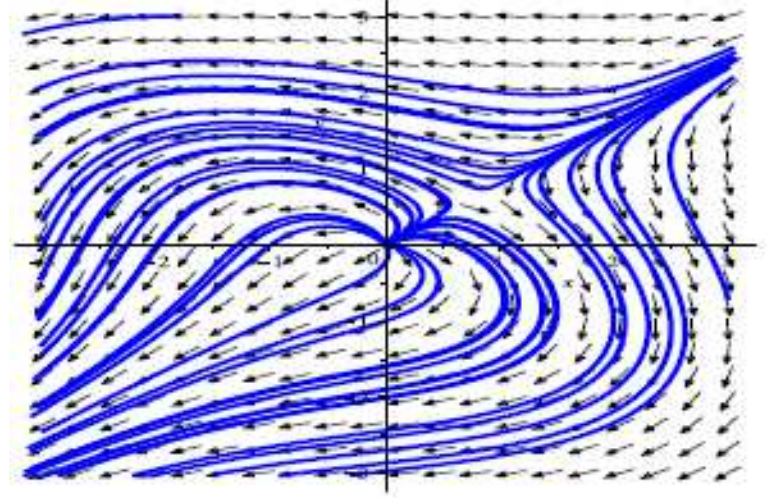
\includegraphics[width=0.55\textwidth]{figure/2_fig1.PNG}
			\caption{The phase portrait for the system in Question 5A.}
		\end{figure}
		%
		critical point is an unstable proper node. Therefore, we cannot make a definite conclusion regarding the relation between the nature of the critical point of the nonlinear system and the corresponding linearisation.\\
		\hspace*{0pt}\hfill\textbf{[3 marks]}\\
		At the critical point $(1/2, 1/2)$, the coefficient matrix of the linearised system is
		$$
		\vb{J}(1/2, 1/2) =
		\begin{pmatrix}
			1 & -2\\
			-2 & 1
		\end{pmatrix},
		$$
		with eigenvalues $r_1 = 3$ and $r_2 = −1$. The eigenvalues are real, with opposite sign. Hence, the critical point is a saddle, which is unstable.
		\hspace*{0pt}\hfill\textbf{[3 marks]}\\
		The phase portrait is shown in Fig. 1. Closer examination reveals that the critical point at the origin is indeed a proper node.\par
		\textbf{(B)} The critical points of the ODE
		$$
		\frac{dr}{dt} = r|r-2|(r-4)
		$$
		are given by $r_1 = 0,\ r_2 = 2$ and $r_3 = 4$.\\
		\hspace*{0pt}\hfill\textbf{[3 marks]}\\
		Note that
		$$
		\frac{dr}{dt} < 0\quad \text{for}\ 0 < r < 4\ \text{and}\ \frac{dr}{dt} > 0\quad \text{for}\ r > 4.
		$$
		The point $r = 0$ corresponds to an asymptotically stable critical point. The critical points $r_2 = 2$ is semistable, whereas the critical point $r_3 = 4$ is unstable.\\
		\hspace*{0pt}\hfill\textbf{[3 marks]}\\
		Since the critical values are isolated, a semistable limit cycle is given by
		$$
		r = 2, \quad \theta = -t + t_0.
		$$
		\hfill\textbf{[2 marks]}\\
		Another periodic solution is found to be
		$$
		r = 4, \quad \theta = -t + t_0,
		$$
		which is unstable.\\
		\hspace*{0pt}\hfill\textbf{[2 marks]}
\end{enumerate}
\end{document}